\documentclass[a4paper,11pt]{jsarticle}


% 数式
\usepackage{amsmath,amsfonts}
\usepackage{bm}
% 画像
\usepackage[dvipdfmx]{graphicx}


\begin{document}

\title{デコーダ回路の設計と制作}
\author{古城隆人}
\date{\today}
\maketitle

\newpage
\section{目的}
電子天秤の制作を行うにあたり、値を表示させるために7セグメントLED1の表示回路を作成する。デコーダ回路の入力は、セレクタ回路から3bitの信号を受け取る。
\section{原理}
実際に回路の制作を行うにあたって使用する部品と動作原理を説明する。
\subsection{ブレッドボード}
ブレッドボードを使用し、デコード回路の作成を行う。この部品はジャンパ線を使用して自由に回路を組み替えれるので、回路の制作に適している。
ブレッドボード上で配線するときはショートしているピンについて理解をしないといけない。
図\ref{fig:breadboard}にブレッドボード写真を示す。
\begin{figure}[h]
  \centering
  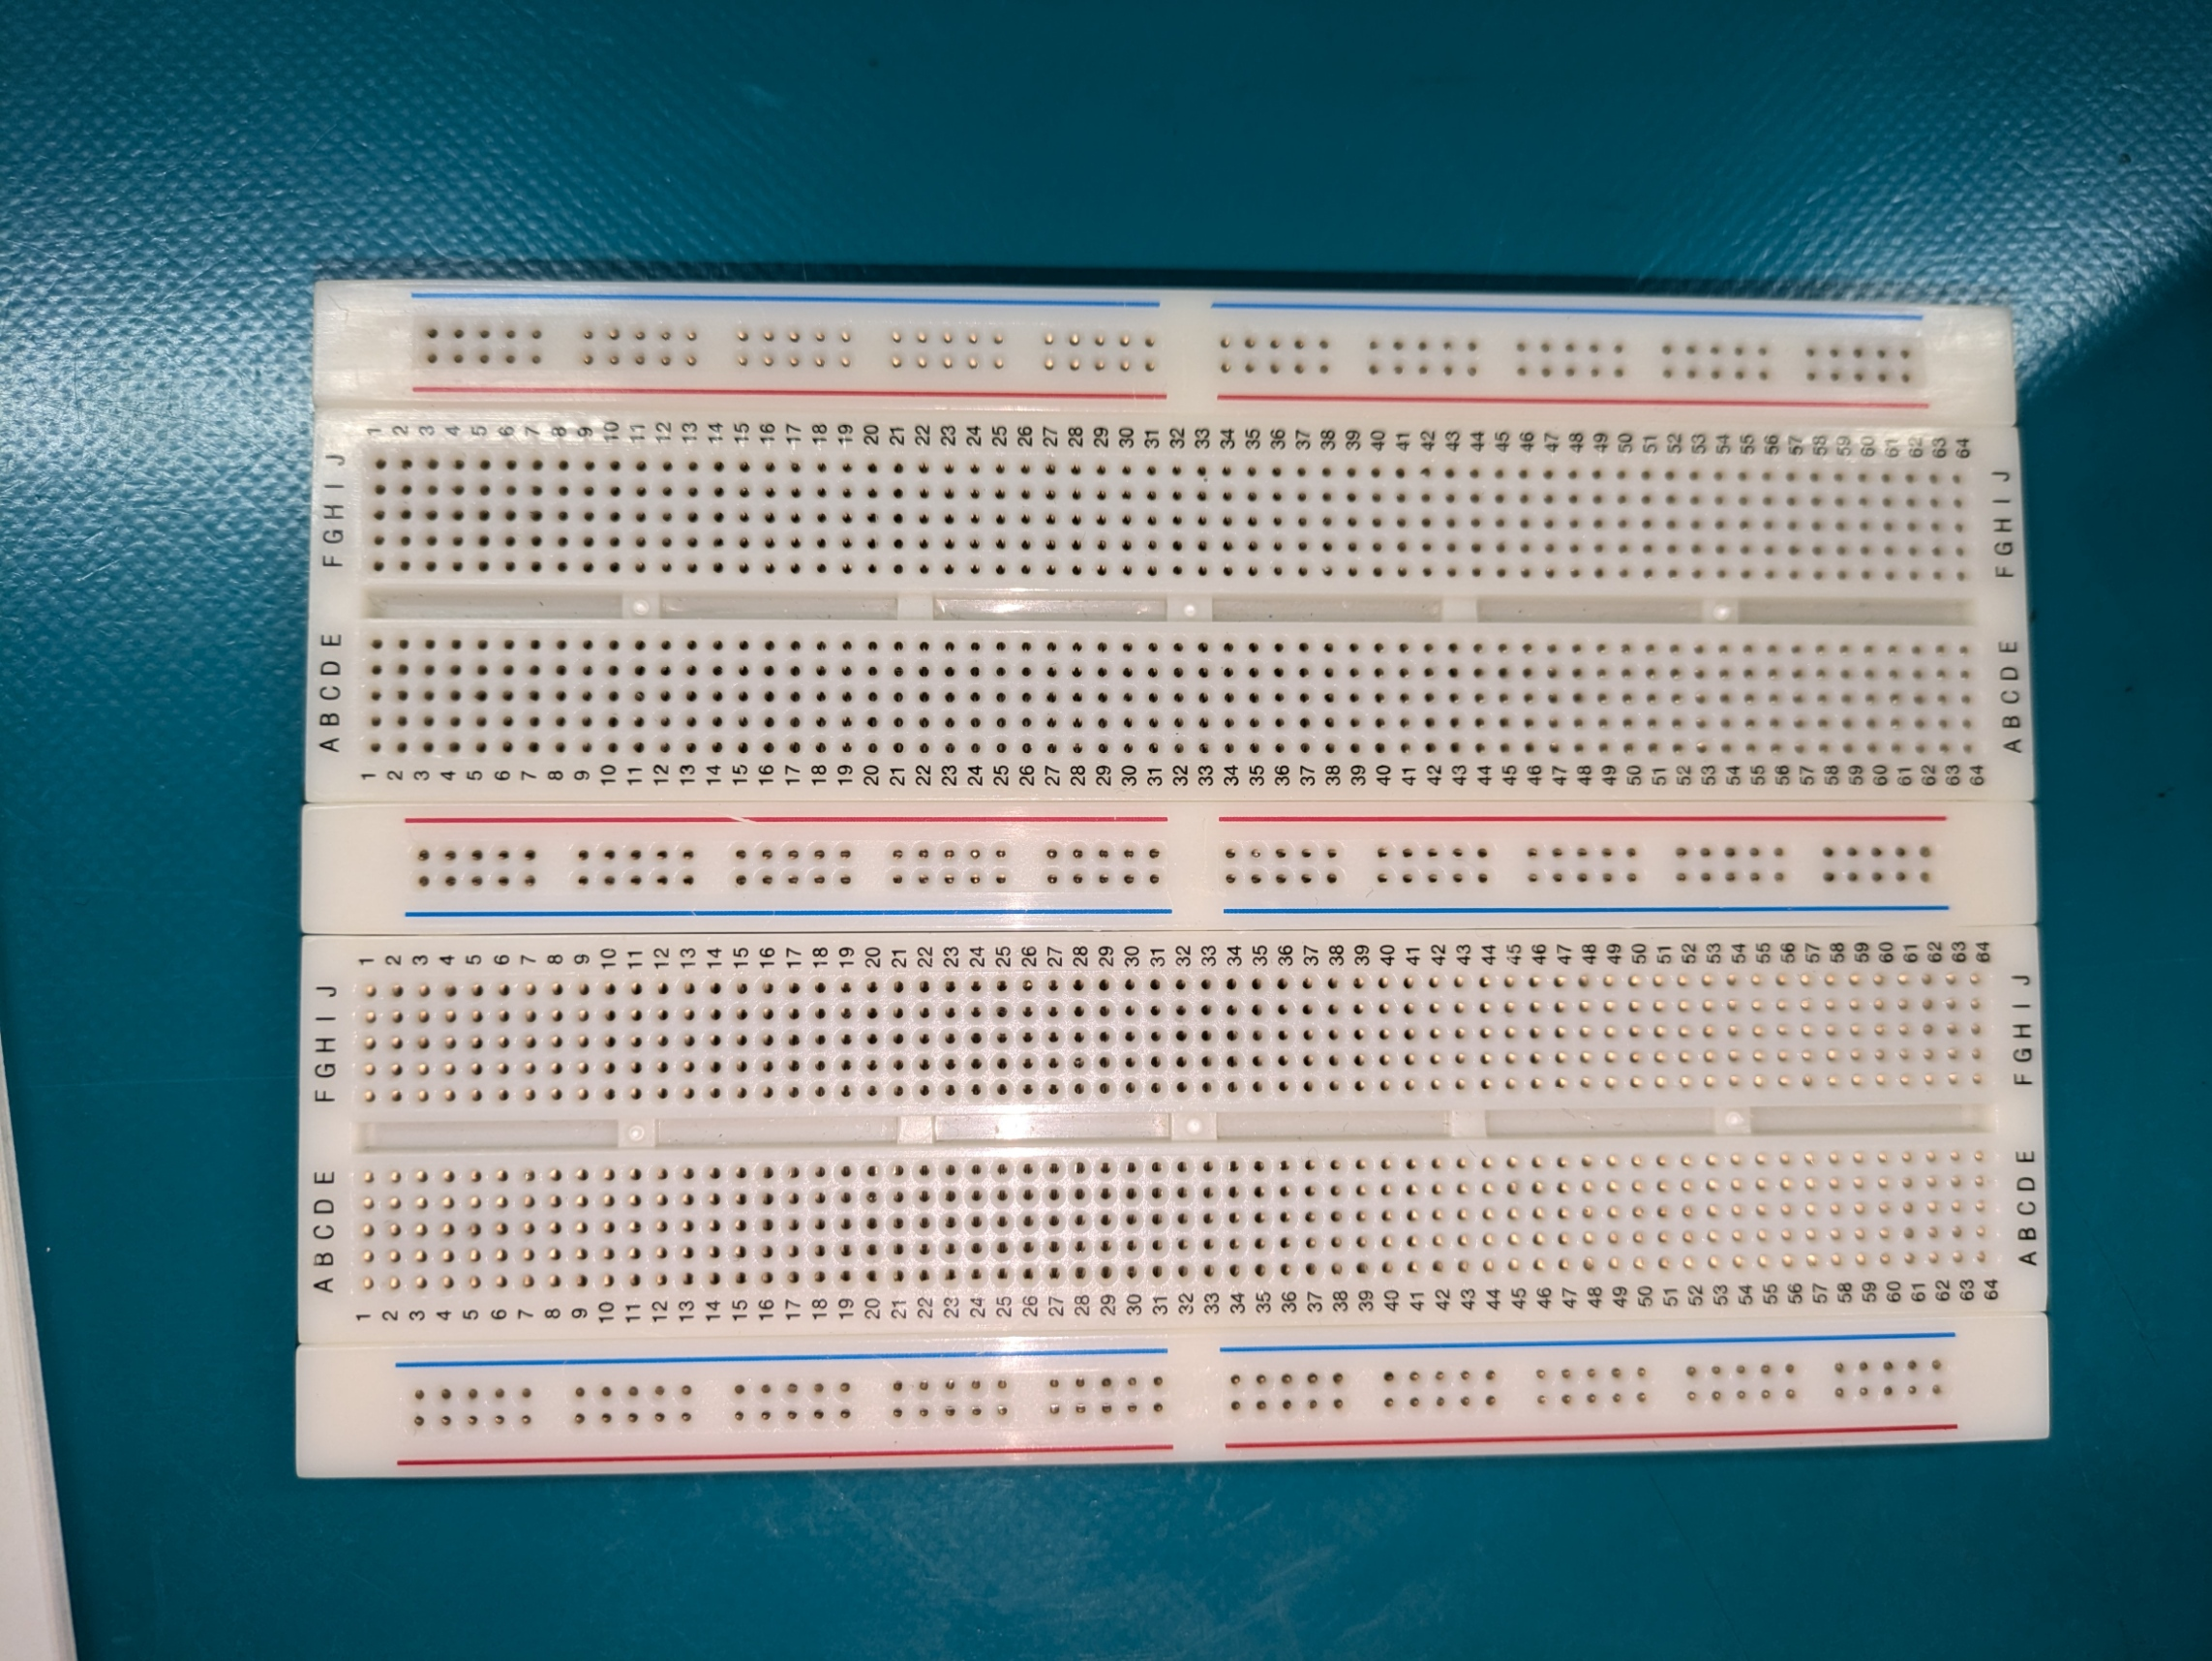
\includegraphics[width=10cm]{./images/breadboard.jpg}
  \caption{ブレッドボードの内部構造}
  \label{fig:breadboard}
\end{figure}
このブレッドボードは5個の部品に分かれており、2この穴が縦に空いてる場所が3個ある。それの間に10個の穴が縦に空いて真ん中に溝がある部品がある。
3個ある横長の部品は内部で電気的に横につながっており、それは青色と赤色の線が横に書いてある穴同士がつながっている。
個の基板では横に2本の線があるので真ん中のピン同士の電気的なつながりはない。この部品は主に電源の端子として使用される。
今回は青色の線が描かれているところを$GND$、赤色の線が描かれているところを$+5V$として使用する。
2個ある長方形の部品は縦にショートしており、5個の穴が内部で電気的につながっている。真ん中の溝で電気的なつながりは切れている。
そのためこのブレッドボードは縦に5個つながっている穴が縦に4個配置されている。この部品は主にIC、ジャンパ線を挿して回路を作成する部品である。
\subsection{7セグメントLED}
7セグメントLEDは7つのLEDを組み合わせたもので、数字を表示させる用途で使用する。7つのLEDはそれぞれaからgまでの名前がついており、それぞれのLEDを点灯させることで数字を表示させる。
7セグメントLEDの略図を図\ref{fig:7seg}に示す。基本的に一番上から時計回りにaからgまでのLEDが配置されている。
\begin{figure}[h]
  \centering
  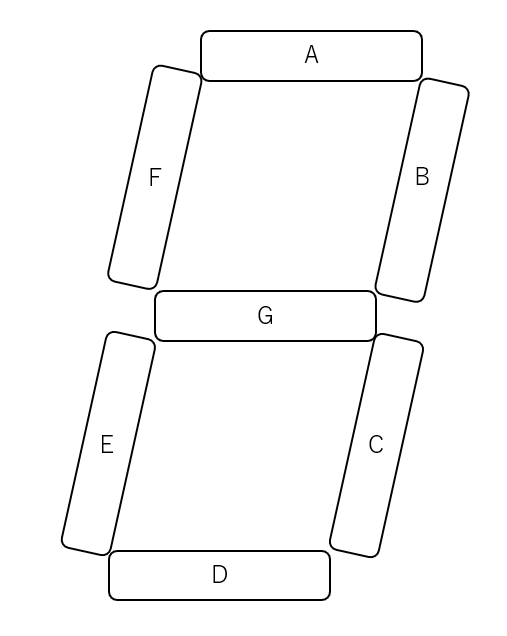
\includegraphics[width=10cm]{./images/7seg.png}
  \caption{7セグメントLEDの略図}
  \label{fig:7seg}
\end{figure}
今回使用するLEDはアノードコモン型の7セグLEDを使用する。アノードコモン型では、その名の通りLEDのアノード端子が共有になっている。
LEDのアノードとは、電流が入力される方向の端子であり、電流を出力する端子をカソードという。アノードからカソードに電流を流すことによりLEDを光らせることが出来る。
そのため、7セグLEDの各LEDの端子とアノードコモンのピンで電圧差が生じたらLEDが光る。アノードコモンのピンには今回は5Vをつなぐため、
各LEDのピンには $GND$ を接続すると光らせることが出来る。
\section{実験方法}

\section{結果}

\section{考察}

\section{付録}


\end{document}